Eingereicht:

\begin{verbatim}[1, 3]\end{verbatim}

Gewählte Option 1 ist verfügbar?\begin{quote}Yes.\end{quote}Gewählte Option 3 ist verfügbar?\begin{quote}Yes.\end{quote}Anmerkungen zur eingereichten Lösung:

Alle angegebenen Klassendiagramme sind korrekt?

\begin{quote}\begin{verbatim}Nein.\end{verbatim}\end{quote}

Die korrekte Lösung ist:\begin{verbatim}[3,4]\end{verbatim}

Ihre Antwort zu Klassendiagramm 1 ist nicht richtig.

Klassendiagramm 1 ist ungültig.

Die Beziehungen in dem Klassendiagramm könnten auf folgende Weise mit Namen versehen werden:



\begin{centering}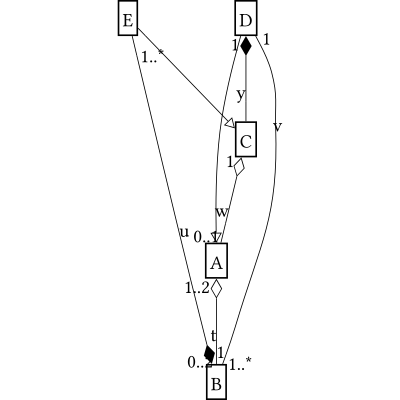
\includegraphics[min width=0.4\textwidth=0.6\textwidth,min height=0.4\textwidth=0.6\textwidth,keepaspectratio,max width=0.9\textwidth,max height=0.9\textwidth]{53/cd304ec9869e94e1ddda9b2aaa917e2b09bc6fc5eb2c530d1213978d80161cb60e01af83b04c596701db35357ce8aed00a3a92e08161.pdf}\end{centering}



Wenn es zum Beispiel Komposition u nicht gäbe, wäre es gültig.

Ihre Antwort zu Klassendiagramm 4 ist nicht richtig.

Klassendiagramm 4 ist gültig.

Die Beziehungen in dem Klassendiagramm könnten auf folgende Weise mit Namen versehen werden:



\begin{centering}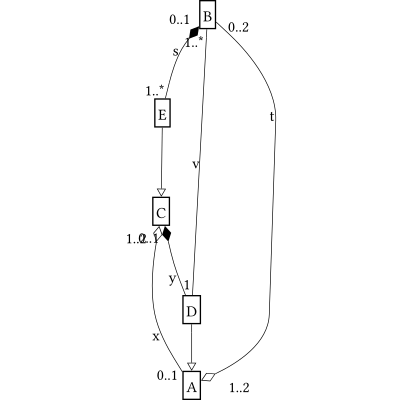
\includegraphics[min width=0.4\textwidth=0.6\textwidth,min height=0.4\textwidth=0.6\textwidth,keepaspectratio,max width=0.9\textwidth,max height=0.9\textwidth]{53/cdf8026e55054824c5b00dbd86a11a47c0e778bb39e7041008f6001317a9eed28f01af83b04c596701db35357ce8aed00a3a92e08161.pdf}\end{centering}



Betrachten Sie nun das folgende Objektdiagramm, welches eine Instanz dieses Klassendiagramms ist:



\begin{centering}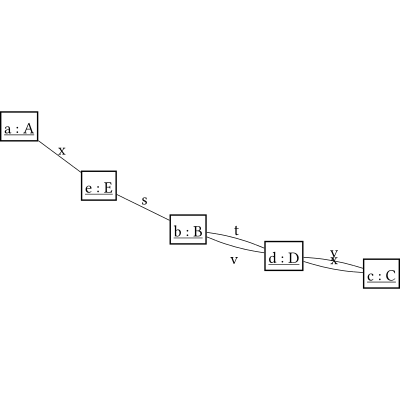
\includegraphics[min width=0.4\textwidth=0.6\textwidth,min height=0.4\textwidth=0.6\textwidth,keepaspectratio,max width=0.9\textwidth,max height=0.9\textwidth]{53/odeb717915f1237f6c1c81d4bbf53a76d1ee08775548a199caba7259f925df238d13.pdf}\end{centering}



